% article.tex
% Submission-ready article for Theoretical Economics Letters (TEL)
% Scientific Research Publishing (SCIRP), ISSN Online: 2162-2086
% https://www.scirp.org/journal/tel/
%
% Compile from Tex/ directory (twice for cross-references; no bibtex pass needed
% because the bibliography is a manual \thebibliography handled by natbib):
%   pdflatex -interaction=nonstopmode article.tex
%   pdflatex -interaction=nonstopmode article.tex
%
% Upload to Overleaf: this file + "Extra images/" folder + the result figures.
% See the \graphicspath note below for the Overleaf figure-placement caveat.

% ---------------------------------------------------------------------------
% DOCUMENT CLASS & GEOMETRY
% ---------------------------------------------------------------------------
\documentclass[a4paper,11pt,twoside]{article}

\usepackage[top=2.4cm, bottom=2.8cm, left=2.2cm, right=2.2cm,
            headheight=14pt]{geometry}

% ---------------------------------------------------------------------------
% PACKAGES
% ---------------------------------------------------------------------------
\usepackage[T1]{fontenc}
\usepackage[utf8]{inputenc}
\usepackage{lmodern}
\usepackage[english]{babel}
\usepackage{microtype}

% Graphics — grffile handles the space in the "Extra images/" directory name.
% On very recent TeX Live the LaTeX kernel handles spaces in file names natively
% and grffile may emit a warning; if so it can be safely removed.
\usepackage{grffile}
\usepackage{graphicx}
% \graphicspath sets two search roots (relative to Tex/ where this file lives):
%   (1) template images in "Extra images/"
%   (2) result figures in ../rl-credit-scoring-sim/artifacts/figures/
% OVERLEAF NOTE: the parent-directory path ("../") is NOT accessible on Overleaf.
% For Overleaf, copy the result PNG(s) into a local "figures/" folder next to
% article.tex and change the second root to {figures/}.
\graphicspath{{Extra images/}{figures/}}

% Tables
\usepackage{booktabs}
\usepackage{tabularx}
\usepackage{array}

% Math
\usepackage{amsmath}
\usepackage{amssymb}

% Colors — Brown section headings (SCIRP style)
\usepackage[dvipsnames]{xcolor}
\definecolor{scirpbrown}{RGB}{101,57,0}

% Section headings in brown small-caps
\usepackage{sectsty}
\allsectionsfont{\color{scirpbrown}\normalfont\scshape\normalsize}
% Make section headings slightly larger than normal text
\sectionfont{\color{scirpbrown}\normalfont\scshape\large}
\subsectionfont{\color{scirpbrown}\normalfont\scshape\normalsize}

% Page headers/footers
\usepackage{fancyhdr}

% Citation wraptable box
\usepackage{wrapfig}
\usepackage{mdframed}

% ---------------------------------------------------------------------------
% BIBLIOGRAPHY STYLE — switchable via a single line (natbib, no bibtex pass).
% The in-text \citet/\citep commands render correctly in BOTH styles, so only
% the one active line below ever needs to change.
% ---------------------------------------------------------------------------
\usepackage[numbers,sort&compress]{natbib}   % NUMERIC style [1] — ACTIVE
%\usepackage[authoryear,round]{natbib}        % AUTHOR-DATE style (Author, Year):
%                                              % uncomment this line and comment
%                                              % the numeric line above to switch.

% Hyperlinks (load after natbib)
\usepackage[colorlinks=true, linkcolor=scirpbrown, citecolor=scirpbrown,
            urlcolor=scirpbrown, bookmarks=true]{hyperref}

% Floats
\usepackage{float}

% Compact lists
\usepackage{enumitem}
\setlist{noitemsep, topsep=3pt}

% ---------------------------------------------------------------------------
% HEADER / FOOTER STYLES
% ---------------------------------------------------------------------------
% First-page style: shows journal banner
\fancypagestyle{first}{%
  \fancyhf{}%
  \fancyhead[L]{%
    
\includegraphics[height=20pt]{index.jpeg}%
    \quad{\small\color{scirpbrown}\textit{Theoretical Economics Letters}, 2026, \textbf{***}, ***-***}% TODO: volume/pages assigned on acceptance
  }%
  \fancyhead[R]{%
    \small\color{scirpbrown}%
    \href{http://www.scirp.org/journal/tel}{\texttt{http://www.scirp.org/journal/tel}}\\
    ISSN Online: 2162-2086%
  }%
  \fancyfoot[C]{\small\color{scirpbrown}\thepage}%
  \renewcommand{\headrulewidth}{0.4pt}%
  \renewcommand{\headrule}{\color{scirpbrown}\hrule width\headwidth height 0.4pt}%
}

% Regular page style
\fancypagestyle{plain}{%
  \fancyhf{}%
  \fancyhead[LE,RO]{\small\color{scirpbrown}E. Baulin, P.\,P. Lukianchenko}%
  \fancyhead[RE,LO]{\small\color{scirpbrown}%
    \textit{Theoretical Economics Letters}}%
  \fancyfoot[C]{\small\color{scirpbrown}\thepage}%
  \renewcommand{\headrulewidth}{0.4pt}%
  \renewcommand{\headrule}{\color{scirpbrown}\hrule width\headwidth height 0.4pt}%
}
\pagestyle{plain}

% ---------------------------------------------------------------------------
% TITLE INFORMATION
% ---------------------------------------------------------------------------
\title{%
  {\color{scirpbrown}\large\scshape
  Reinforcement Learning vs.\ Rule-Based Policies\\[4pt]
  for Dynamic Credit Threshold Control:\\[4pt]
  A Simulation Study}%
}

\author{%
  Evgeny Baulin\textsuperscript{1} \quad P.\,P.\ Lukianchenko\textsuperscript{2}\\[4pt]
  {\small \textsuperscript{1}Faculty of Computer Science, Bachelor's Programme
   ``Data Science and Business Analytics'',}\\
  {\small National Research University Higher School of Economics, Moscow, Russia}\\[2pt]
  {\small \textsuperscript{2}Big Data and Information Retrieval School,
   National Research University Higher School of Economics, Moscow, Russia}\\[3pt]
  {\small Corresponding author:
   \href{mailto:e.baulin@icloud.com}{\texttt{e.baulin@icloud.com}}}%
}
\date{}

% ---------------------------------------------------------------------------
% DOCUMENT BEGIN
% ---------------------------------------------------------------------------
\begin{document}

\thispagestyle{first}
\maketitle
\vspace{-1.5em}

% ---------------------------------------------------------------------------
% CITATION / LICENCE BOX (left-hand wraptable, SCIRP style)
% ---------------------------------------------------------------------------
\noindent\begin{minipage}{0.46\textwidth}
  \begin{mdframed}[%
      linecolor=scirpbrown, linewidth=0.8pt,
      innertopmargin=6pt, innerbottommargin=6pt,
      innerleftmargin=6pt, innerrightmargin=6pt,
      backgroundcolor=white]
    {\footnotesize
      \textbf{How to cite this paper:}\\[2pt]
      Baulin, E., \& Lukianchenko, P.\,P. (2026). Reinforcement
      Learning vs.\ Rule-Based Policies for Dynamic Credit Threshold
      Control: A Simulation Study.
      \textit{Theoretical Economics Letters},
      \textbf{**}, **-**.\\[4pt] % TODO: volume/pages on acceptance
      \texttt{https://doi.org/10.4236/tel.2026.*****}\\[6pt] % TODO: DOI on acceptance
      \textbf{Received:} May 30, 2026\\
      \textbf{Accepted:} *** ***, 2026\\ % TODO
      \textbf{Published:} *** ***, 2026\\[6pt] % TODO
      \begin{minipage}[c]{0.48\linewidth}
        
\includegraphics[height=14pt]{ccby40.png}
      \end{minipage}%
      \begin{minipage}[c]{0.48\linewidth}
        
\includegraphics[height=14pt]{openaccess.jpg}
      \end{minipage}\\[2pt]
      Copyright \copyright\ 2026 by author(s) and\\
      Scientific Research Publishing Inc.\\
      This work is licensed under the Creative\\
      Commons Attribution International License\\
      (CC BY 4.0).\\
      {\small\ttfamily\raggedright http://creativecommons.org/\linebreak licenses/by/4.0/}%
    }
  \end{mdframed}
\end{minipage}
\vspace{0.8em}

% ---------------------------------------------------------------------------
% ABSTRACT
% ---------------------------------------------------------------------------
\begingroup\tolerance=9999\emergencystretch=12pt\relax
{\color{scirpbrown}\rule{\linewidth}{1.4pt}}\\[2pt]
\noindent\textbf{\color{scirpbrown}\scshape Abstract}\\[4pt]
\noindent
Portfolio-level credit acceptance thresholds are revised periodically in practice,
making the decision sequential rather than one-shot: each week the controller
sets two acceptance thresholds---one for new clients and one for repeat clients---and
then observes delayed repayment and default outcomes over subsequent weeks.
We evaluate six deep reinforcement learning (RL) algorithms---DQN, Double-DQN, PPO,
SAC, A3C, and A2C---against five rule-based baselines in a calibrated synthetic
credit-portfolio simulator across six market scenarios and four observation-space
sizes (12D, 20D, 30D, 50D).
The simulator is a calibrated proof-of-concept test bench, not a substitute for real
banking data; only observation dimensionality varies across the four conditions, with
the simulator, reward, seeds, and evaluation protocol held fixed.
We find that the constraint-aware weekly policy is the best overall controller by
cumulative reward (the primary ranking metric; realized profit 3{,}802{,}547) and is
statistically tied with the profit-oriented policy on realized profit; no RL agent
wins any scenario by reward or profit.
Double-DQN is the strongest RL agent, peaking at 12D (realized profit 3{,}446{,}564)
and declining at higher state dimensionality.
Richer-state RL agents nonetheless achieve lower portfolio default rates than the two
profit-seeking baselines in a majority of scenarios---while the risk-aware weekly policy
remains the lowest-default controller overall---a conditional risk-side advantage.
We conclude that well-designed rule-based weekly threshold search remains the benchmark
when training budgets are short.
  {\color{scirpbrown}\rule{\linewidth}{0.8pt}}
\endgroup

% ---------------------------------------------------------------------------
% KEYWORDS
% ---------------------------------------------------------------------------
\noindent\textbf{\color{scirpbrown}Keywords}\\[2pt]
\noindent
Reinforcement Learning; Credit Scoring; Threshold Control; Markov Decision Process;
Delayed Rewards; Portfolio Simulation; Rule-Based Policies; State Dimensionality

% ---------------------------------------------------------------------------
\clearpage
% ---------------------------------------------------------------------------

% ===========================================================================
\section{Introduction}
% ===========================================================================

Banks and consumer-lending institutions revise acceptance thresholds periodically
rather than once: what fraction of applicants to approve this week depends on the
current portfolio composition, outstanding capital commitments, rolling default
rates, and market conditions that evolve between decisions.
The academic literature has largely treated threshold selection as a one-shot
classification problem---estimate default probability, choose a cut-off, evaluate
by AUC or Gini---ignoring the sequential nature of actual threshold management
\citep{thomas2017, lessmann2015}.
That gap between static cut-off optimisation and dynamic portfolio management
motivates the present study.

Reinforcement learning (RL) provides a natural framework for decisions with delayed
consequences \citep{sutton2018}.
An RL agent observes the state of the portfolio, selects a pair of
weekly thresholds, and receives a reward signal that reflects realized portfolio
cash flows rather than immediate cohort expectations.
The delayed-outcome setting is central: a loan accepted at week $t$ may not default
or repay until week $t + \Delta$, so the correct evaluation object is the full
portfolio trajectory, not the immediately observable cohort.
\citet{herasymovych2019} demonstrated that a DQN agent can
learn to adjust a single acceptance threshold in a simulated credit environment
with delayed outcomes, establishing the structural ideas on which this study builds.

\textbf{Calibration disclaimer.}\;
All experiments in this paper use a synthetic simulator calibrated to published
retail lending statistics (Bank of Russia supervisory data and ECB SSM loan loss
reports) as a controlled proof-of-concept test bench.
Synthetic simulation is standard practice in RL-based credit research because
real loan-level panels with weekly cohort granularity and observable repayment
and default events are not publicly available \citep{herasymovych2019, lessmann2015}.
The simulator provides full control over market regime, segment composition, and
shock timing, making the multi-scenario robustness evaluation possible.
Results should be interpreted as evidence about algorithmic behaviour under these
controlled conditions, not as forecasts for any specific production portfolio.

The paper extends the framework of \citet{herasymovych2019}
with four contributions: (i) split weekly thresholds for new and repeat client
segments; (ii) a controlled state-dimensionality experiment comparing 12D, 20D,
30D, and 50D observation sizes under a fixed protocol; (iii) five economically
meaningful rule-based baselines as the comparison standard; and (iv) statistical
hypothesis tests on paired run-level data.
The central research question is:
\begin{quote}
  \emph{Under which conditions does reinforcement learning provide a robust improvement
    over rule-based threshold policies in a delayed-outcome credit-scoring environment?}
\end{quote}
The short answer the data provide is nuanced: strong rule-based weekly search wins
every scenario and dimension by headline metrics, but richer-state RL agents produce
lower portfolio default rates than the profit-seeking baselines in a majority of
scenarios (the risk-aware weekly policy stays the lowest overall), indicating a conditional
risk-side advantage that becomes visible once the profit ranking is supplemented
by credit-quality metrics.

The code, data, and experiment configuration are publicly available at
\url{https://github.com/EvgenyBaulin/Evaluation-of-RL-framework-in-a-credit-scoring-problem}.

% ===========================================================================
\section{Related Work}
% ===========================================================================

\subsection{Credit Scoring, Thresholds, and Portfolio Risk}

Traditional credit scoring estimates default probability at the application level
and selects a cut-off that balances interest income against expected loss
\citep{thomas2017, hand1997, siddiqi2006}.
Benchmarking studies have shown that classifier rankings depend on the dataset
and evaluation protocol, and that logistic regression and gradient-boosted trees
are difficult to outperform with more complex classifiers \citep{lessmann2015, baesens2003}.
A closely related line of work treats threshold choice as a cost-sensitive economic
decision rather than a classification tuning step \citep{baesens2003}.
\citet{bellotti2009} note that under Basel\,II/III capital
adequacy requirements, the threshold affects outstanding exposure, realized losses,
and regulatory capital in ways that make static cut-off selection insufficient when
market conditions or portfolio composition drift over time.

\subsection{Reinforcement Learning for Sequential Decisions}

Reinforcement learning addresses problems with delayed consequences via the Markov
Decision Process (MDP) framework \citep{sutton2018, dayan2008}.
Key deep RL algorithms used in this study are: DQN \citep{mnih2015dqn}, whose
experience-replay mechanism provides off-policy sample efficiency on discrete action
spaces; Double DQN \citep{van2016ddqn}, which reduces the overestimation bias of
vanilla DQN; PPO \citep{schulman2017ppo}, an on-policy policy-gradient method with
stable monotonic updates; SAC \citep{haarnoja2018sac}, an off-policy maximum-entropy
actor-critic; and A3C/A2C \citep{mnih2016a3c}, asynchronous and synchronous
actor-critic variants.
Implementations use Stable-Baselines3 \citep{stable_baselines3}.
A comprehensive survey of deep RL methods appears in \citet{arulkumaran2017}.

\subsection{Research Gap}

The direct precursor \citep{herasymovych2019} compared a DQN agent with a static
threshold in a single scenario using a shared (non-split) threshold.
No prior work has simultaneously evaluated (1) split thresholds for distinct
borrower segments, (2) controlled observation-dimensionality comparison,
(3) strong economically motivated rule-based baselines, and (4) six market
scenarios with statistical testing---the combination that defines the
contribution of this paper.

% ===========================================================================
\section{Problem Formulation and Methodology}
% ===========================================================================

\subsection{MDP Formulation}

We model the weekly threshold-control problem as a discrete-time MDP
$(\mathcal{S}, \mathcal{A}, \mathcal{P}, r, \gamma)$.
The \textbf{state} $s_t \in \mathbb{R}^d$ ($d \in \{12, 20, 30, 50\}$) is a
portfolio summary vector observed at the beginning of interactive week $t$.
It includes approval rates, default rates, realized profit and NPV, capital usage,
outstanding exposure, segment shares, and (at higher dimensionalities) lagged and
rolling history.
The \textbf{action} is a pair of acceptance thresholds
$a_t = (\tau^{\text{new}}_t, \tau^{\text{repeat}}_t) \in \{35, 40, \ldots, 85\}^2$:
applications from new (repeat) clients with credit score above
$\tau^{\text{new}}_t$ ($\tau^{\text{repeat}}_t$) are accepted.
This yields $11 \times 11 = 121$ joint actions per week.
The \textbf{reward} is described in Section~\ref{sec:reward}.
The discount factor is $\gamma = 0.99$.

\subsection{Simulation Environment}

\textit{Note on synthetic data.}\;
As stated in the Introduction, the simulator is a calibrated synthetic
test bench used because real weekly cohort-level loan data with observable
delayed repayment and default events is not publicly available.

Each episode consists of three phases.
(1) An \textbf{8-week warm-up} pre-fills the loan book using default thresholds
before the controller begins acting.
(2) During the \textbf{52-week interactive horizon} the controller sets weekly
thresholds; the simulator generates applications from Beta-distributed credit
scores for new and repeat segments, applies a logistic default-probability mapping,
accepts loans above the threshold, and schedules repayment/default/recovery events
in a forward event queue.
(3) \textbf{Terminal settlement} resolves all pending cash flows at episode end
so that loans originated near the horizon are not mechanically penalized.
Default probabilities are calibrated to target 4--6\% in the base scenario and
9--14\% under adverse stress, consistent with published retail lending statistics.
Six market scenarios stress specific portfolio-management weaknesses: stable baseline,
score drift, abrupt adverse shock, class-imbalance shift, noisy observations, and
divergent new/repeat segment dynamics (Table~\ref{tab:scenarios}).

\begin{table}[t]
  \centering
  \small
  \caption{The six evaluation scenarios and their primary stress mechanism.}
  \label{tab:scenarios}
  \begin{tabularx}{0.96\linewidth}{>{\ttfamily}p{0.26\textwidth}X}
    \toprule
    Scenario                & Stress mechanism                                               \\
    \midrule
    base\_market            & Stable; cleanest test of policy signal exploitation            \\
    drift                   & Gradual new-client score deterioration and rising defaults     \\
    adverse\_stress         & Abrupt shock: higher defaults, larger loans, capital pressure  \\
    class\_imbalance\_shift & Growing share of weaker new applicants; tests composition risk \\
    noise                   & Stable mean with noisy weekly volumes and measurements         \\
    split\_policy\_dynamics & New clients deteriorate while repeat clients improve           \\
    \bottomrule
  \end{tabularx}
\end{table}

\subsection{Agents and Baselines}

\textbf{RL agents.}\;
All six agents use a shared two-layer MLP ($2 \times 64$ hidden units) and
Stable-Baselines3 default hyperparameters (see Appendix~\ref{app:hyperparams}).
No hyperparameter search is performed; the deliberate intent is to isolate the
state-dimensionality signal rather than optimise the training recipe.

\textbf{Rule-based baselines} span five management styles.
The static-threshold baseline (\texttt{static\_threshold}) applies one fixed shared
threshold.
The split-static baseline (\texttt{split\_policy\_static}) maintains separate fixed
defaults per segment.
The profit-oriented policy (\texttt{profit\_oriented}) performs a weekly grid search
maximising current-cohort expected profit without penalty terms.
The risk-aware weekly policy (\texttt{risk\_aware\_weekly}) adjusts thresholds
reactively to rolling default pressure and capital signals.
The constraint-aware weekly policy (\texttt{constraint\_aware\_weekly}) runs a
penalty-weighted weekly grid search that explicitly internalises default-rate,
approval-rate, capital-usage, and volatility violations.

\subsection{Reward Function}
\label{sec:reward}

With delayed reward enabled, the shaped weekly reward is:
\begin{equation}
  \label{eq:reward}
  \begin{aligned}
    r_t ={} & \;
    w_p\,\Pi^{\text{realized}}_t
    + w_n\,\mathrm{NPV}^{\text{realized}}_t
    - w_s\,\hat{d}_t \cdot 100                                                                   \\
            & - \lambda_d\!\left[\max\!\bigl(0,\,\bar{d}_t - 0.12\bigr)\right]^{\!2}\!\cdot 1000
    - \lambda_a\left|\alpha_t - 0.42\right|\cdot 1000                                            \\
            & - \lambda_c\!\left[\max\!\bigl(0,\,c_t - 0.82\bigr)\right]^{\!2}\!\cdot 1000
    - \lambda_v\max\!\!\left(0,\,\frac{\sigma_{\Pi,t}-8500}{8500}\right)\!\cdot 1000,
  \end{aligned}
\end{equation}
where $\Pi^{\text{realized}}_t$ and $\mathrm{NPV}^{\text{realized}}_t$ are realized
weekly profit and NPV (not current-cohort expectations), $\hat{d}_t$ is the expected
default rate of the current cohort, $\bar{d}_t$ is the rolling realized default rate,
$\alpha_t$ is the weekly approval rate, $c_t$ is the projected capital usage ratio, and
$\sigma_{\Pi,t}$ is realized profit volatility.
The four constants are calibration targets: the default-rate cap ($0.12$), the
target approval rate ($0.42$), the capital-usage cap ($0.82$), and the
profit-volatility scale ($8500$).
Active weights: $w_p{=}1.0$, $w_n{=}0.25$, $w_s{=}0.35$, $\lambda_d{=}9.0$,
$\lambda_a{=}2.0$, $\lambda_c{=}3.5$, $\lambda_v{=}1.4$.

The reward is deliberately multi-objective.
Rankings by cumulative reward need not coincide with rankings by raw profit
(which is intentional: the reward encodes portfolio risk constraints, not
profit alone).
Throughout this paper, ``realized profit'' is computed from realized interactive
weekly profits plus terminal settlement---that is, realized final portfolio profit
rather than a current-cohort expectation.

% ===========================================================================
\section{Experimental Design}
% ===========================================================================

The experiment is fully controlled: \emph{only} observation dimensionality varies
across the four runs; everything else---simulator, reward, the eight random seeds,
50 training episodes per seed, evaluation protocol, scenarios, threshold grid, and
controller set---is held fixed.
The full-profile scale used to generate the main summary tables is
6~agents~$\times$~4~dimensions~$\times$~6~scenarios~$\times$~8~seeds~$= 1{,}152$
training runs, with 576 evaluation runs per controller per dimension.
A validity layer programmatically verifies that the first 12 observation features are
bit-for-bit identical across all four state sizes on a common reset and three
fixed-action transitions.

The four observation layers are constructed cumulatively (Table~\ref{tab:state-layers}).
Each layer adds features that a portfolio manager would realistically observe
at weekly decision time, with no access to future outcomes.

\begin{table}[t]
  \centering
  \small
  \caption{Cumulative observation layers. The first 12 features are invariant across
    all configurations and are verified programmatically before each experiment.}
  \label{tab:state-layers}
  \begin{tabularx}{0.96\linewidth}{>{\centering\arraybackslash}p{0.06\textwidth}
      >{\raggedright\arraybackslash}X}
    \toprule
    Size & Added information                                                             \\
    \midrule
    12D  & Compact dashboard: week progress, overall/segment approval rates,
    rolling realized default rate, expected default rate, realized profit, profit
    volatility, projected capital usage, outstanding ratio, both threshold levels.       \\
    20D  & 12D~+ current economic context: repeat segment share, expected profit/NPV per
    application, realized NPV, weekly reward, threshold gap, capital headroom,
    realized-vs-expected default gap.                                                    \\
    30D  & 20D~+ lagged/rolling memory: second-lag approval/default/profit/capital,
    four-week rolling means and std of approval, default, and profit, lagged
    threshold changes.                                                                   \\
    50D  & 30D~+ segment-specific signals and stability descriptors: segment approval/
    default/profit indicators, accepted-share ratios, rolling reward moments,
    cumulative reward/profit to date, capital-usage volatility, outstanding-ratio
    changes, threshold-gap history, application-volume ratio.                            \\
    \bottomrule
  \end{tabularx}
\end{table}

\subsection{Hypotheses}
\label{sec:hypotheses}

Three hypotheses are stated in advance of the results and tested on paired
run-level data in Section~\ref{sec:stat-tests}.
\begin{description}[leftmargin=2.2em,style=nextline]
  \item[H1 (State representation).] Richer state representations improve the best RL
        frontier from 12D to 30D, while the move from 30D to 50D does not necessarily
        create additional improvement.
  \item[H2 (RL vs.\ rule-based).] RL improves over rule-based policies only in some
        scenarios and metrics; the universal claim that RL robustly dominates strong
        rule-based baselines is expected to be \emph{rejected}.
  \item[H3 (Delayed evaluation).] Early-period performance is an unreliable proxy for
        final realized portfolio quality when outcomes are delayed and terminal settlement
        is applied---the ``locally worse, globally better'' pattern is expected to hold.
\end{description}

% ===========================================================================
\section{Results}
% ===========================================================================

\subsection{Best Overall and Best RL Controller by Dimension}

Table~\ref{tab:best-by-dim} reports the strongest controller when baselines and RL
agents are pooled under the repository's official ranking rule (highest cumulative
reward, then highest profit, then lowest default rate), and separately the strongest
RL controller in each dimension (full-profile run, 8 seeds $\times$ 50 episodes per
seed; see the public repository for data and configuration).
Figure~\ref{fig:saturation} visualises the same comparison.

\begin{table}[t]
  \centering
  \small
  \caption{Best overall controller and best RL controller by state dimension
    (full-profile run). The baseline line is flat because the leading baseline does
    not depend on the RL observation vector. ``Profit'' is realized final portfolio
    profit (Section~\ref{sec:reward}); ``Reward'' is cumulative shaped reward.}
  \label{tab:best-by-dim}
  \setlength{\tabcolsep}{4pt}
  \begin{tabular}{c l l r r r}
    \toprule
    Dim & Controller              & Type     & Profit        & Reward        & Default rate \\
    \midrule
    \multicolumn{6}{l}{\textit{Best overall (pooled, by cumulative reward)}}                \\
    12  & Constraint-aware weekly & baseline & 3{,}802{,}547 & 3{,}666{,}052 & 0.0760       \\
    20  & Constraint-aware weekly & baseline & 3{,}802{,}547 & 3{,}666{,}052 & 0.0760       \\
    30  & Constraint-aware weekly & baseline & 3{,}802{,}547 & 3{,}666{,}052 & 0.0760       \\
    50  & Constraint-aware weekly & baseline & 3{,}802{,}547 & 3{,}666{,}052 & 0.0760       \\
    \midrule
    \multicolumn{6}{l}{\textit{Best RL agent}}                                              \\
    12  & Double-DQN              & RL       & 3{,}446{,}564 & 3{,}449{,}745 & 0.0756       \\
    20  & Double-DQN              & RL       & 3{,}124{,}322 & 3{,}281{,}011 & 0.0694       \\
    30  & Double-DQN              & RL       & 3{,}172{,}605 & 3{,}311{,}519 & 0.0725       \\
    50  & Double-DQN              & RL       & 3{,}034{,}292 & 3{,}196{,}350 & 0.0700       \\
    \bottomrule
  \end{tabular}
\end{table}

\begin{figure}[t]
  \centering
  % NOTE: cosmetic mismatch — the baked-in PNG title reads "full profile" (unhyphenated)
  % while this caption uses "full-profile". Regenerate the figure to hyphenate the title;
  % the LaTeX caption below is the authoritative, hyphenated form.
  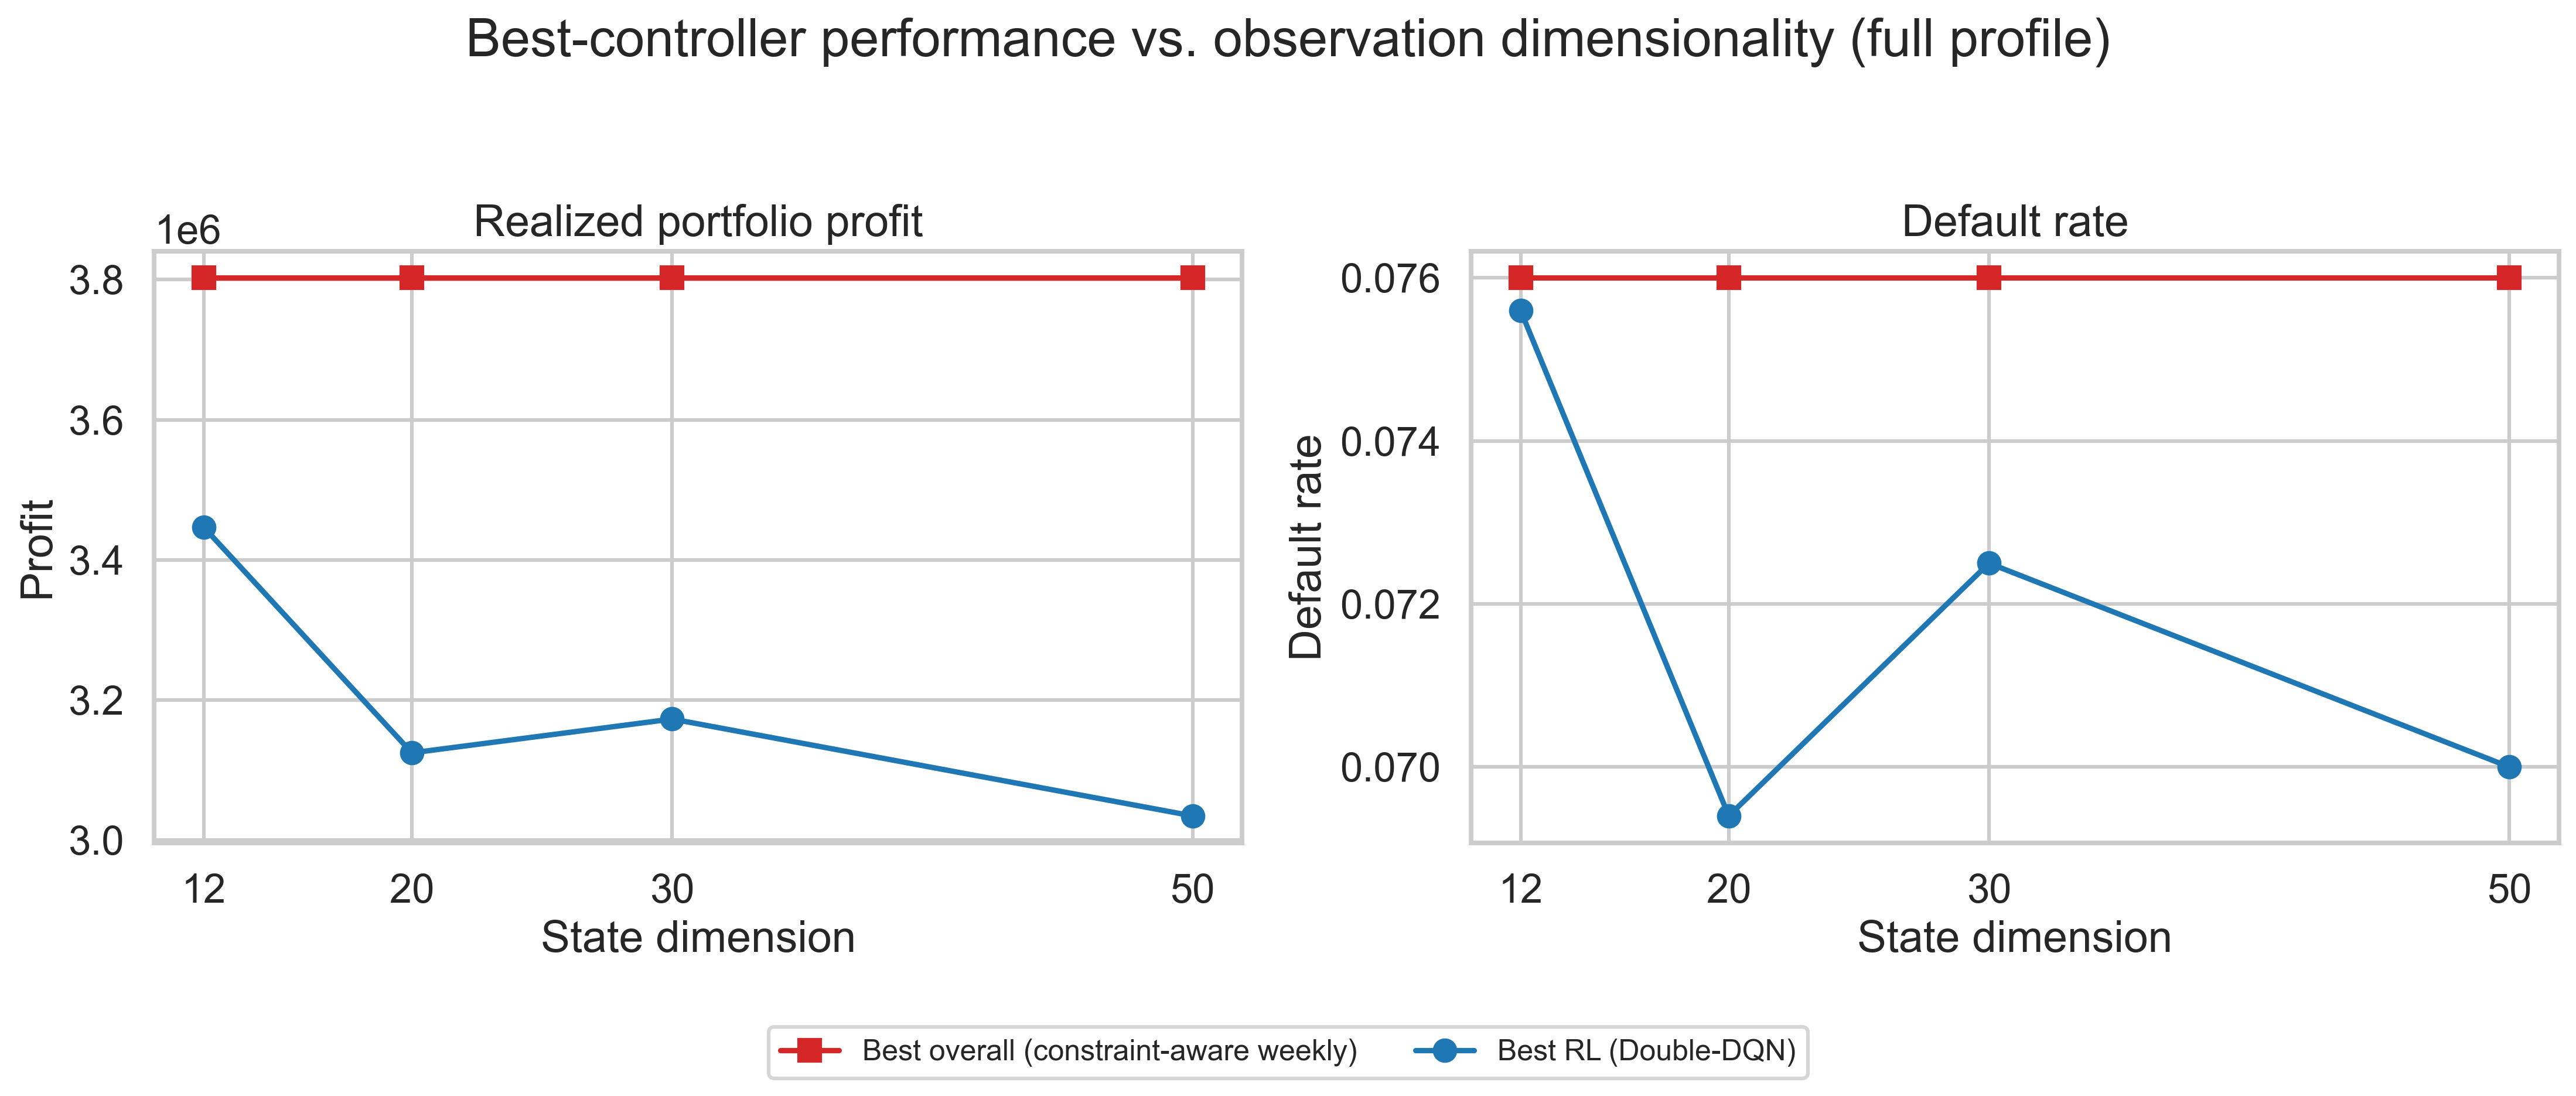
\includegraphics[width=0.98\linewidth]{dimensionality_saturation.png}
  \caption{Best-controller performance versus observation dimensionality
    (full-profile run, 8 seeds). \textit{Left}: realized portfolio profit;
    \textit{right}: default rate. The best overall controller (the constraint-aware
    weekly policy) is independent of the RL state vector and is therefore flat across
    dimensions, while the best RL agent (Double-DQN) peaks at 12D on profit and then
    declines---a saturation-and-regression pattern rather than monotone improvement.}
  \label{fig:saturation}
\end{figure}

By cumulative reward---the primary ranking metric---the constraint-aware weekly
policy is the best overall controller in every dimension (reward 3{,}666{,}052).
On raw realized profit it is statistically tied with the profit-oriented policy,
which is marginally higher (3{,}803{,}168 vs.\ 3{,}802{,}547); the two differ by
less than $0.02\%$ and the difference is not economically meaningful.
The flat baseline row is the cleanest evidence that the experiment successfully
isolates the effect of observation size on RL quality: the leading rule-based policy
is independent of the RL state vector by construction.
The best RL profit peaks at 12D and declines---a \emph{saturation and regression}
pattern, not a monotone improvement---with the 12D$\to$20D drop of $-$322{,}241
being the sharpest.
Default rate for Double-DQN improves from 7.56\% at 12D to 6.94\% at 20D, rises to
7.25\% at 30D, and settles at 7.00\% at 50D, suggesting that the risk-side benefit of
additional features has a different shape than the profit benefit.
At 12D, the gap between the best RL and the best overall controller is
$-$355{,}983 ($-$9.4\% in profit), a meaningful but not catastrophic shortfall.

\subsection{Agent Comparison}

Table~\ref{tab:agent-summary} summarises the mean performance of each agent across
all four dimensions, alongside the three principal rule-based baselines
(full-profile run).

\begin{table}[t]
  \centering
  \small
  \caption{Agent and baseline summary (mean across all four dimensions, full-profile
    run). A3C and A2C are reported in a single combined row.
    ``Approval'' denotes mean weekly approval rate.}
  \label{tab:agent-summary}
  \begin{tabular}{l l r r r}
    \toprule
    Controller              & Type     & Mean profit   & Default rate & Approval  \\
    \midrule
    Constraint-aware weekly & baseline & 3{,}802{,}547 & 7.60\%       & $\dagger$ \\ % TODO: full-profile approval-rate aggregate for this baseline not in released summary
    Profit-oriented         & baseline & 3{,}803{,}168 & $\dagger$    & $\dagger$ \\ % TODO: full-profile default/approval aggregates for this baseline not in released summary
    Static-threshold        & baseline & $\dagger$     & $\dagger$    & $\dagger$ \\ % TODO: full-profile profit/default/approval aggregates for this baseline not in released summary
    \midrule
    Double-DQN              & RL       & 3{,}194{,}446 & 7.19\%       & 0.767     \\
    DQN                     & RL       & 2{,}960{,}000 & 7.02\%       & 0.700     \\
    PPO                     & RL       & 2{,}620{,}000 & 6.21\%       & 0.572     \\
    SAC                     & RL       & 1{,}820{,}000 & 6.63\%       & 0.449     \\
    A3C / A2C (avg)         & RL       & 2{,}470{,}000 & 6.60\%       & 0.570     \\
    \bottomrule
  \end{tabular}\par
  \vspace{2pt}
  {\footnotesize $\dagger$~Per-controller full-profile default- and approval-rate
    aggregates for the rule-based baselines (and the static-threshold profit) are not
    included in the released full-profile summary and are omitted rather than estimated.
    RL per-agent profit means are shown at the precision of the released aggregates;
    the Double-DQN mean is computed exactly from its four per-dimension values.}
\end{table}

Double-DQN leads all RL agents on profit (3{,}194{,}446) and closely matches the
top baselines' approval rate (76.7\%), but still falls 9.4\% short of the best
baseline at its 12D peak.
PPO stands out for its low default rate (6.21\%) despite moderate profit, and
is numerically identical across 12D, 20D, 30D, and 50D.
This is itself a finding: under the modest training budget PPO converges to a
degenerate, essentially constant-threshold policy (consistent with the near-zero
threshold volatility reported in Section~\ref{sec:episode-static}), so the additional
observation features are effectively unused rather than informative.
SAC is the weakest RL agent overall and deteriorates further at 50D.

\subsection{Scenario-Level Winners}

Table~\ref{tab:scenario-winners} reports the reward-based, profit-based, and
lowest-default-rate winner for each scenario at the 50D configuration.
The table illustrates why a single-metric ranking is insufficient.

\begin{table}[t]
  \centering
  \small
  \caption{Scenario-level winners at 50D state (full-profile run; the same
    qualitative pattern holds at 12D/20D/30D, shown here for 50D).
    \textit{Reward winner}: highest cumulative shaped reward.
    \textit{Profit winner}: highest realized profit.
    \textit{Default winner}: lowest default rate. No RL agent wins any scenario by
    reward or profit. The risk-aware weekly policy is the single lowest-default
    controller in every scenario; the best RL agent nonetheless undercuts both
    profit-seeking baselines (the profit-oriented and constraint-aware weekly policies)
    on default rate in a majority of scenarios.}
  \label{tab:scenario-winners}
  \setlength{\tabcolsep}{4pt}
  \begin{tabular}{>{\ttfamily}l l l l}
    \toprule
    Scenario                & Reward winner           & Profit winner           & Default winner    \\
    \midrule
    adverse\_stress         & Static-threshold        & Constraint-aware weekly & Risk-aware weekly \\
    base\_market            & Profit-oriented         & Profit-oriented         & Risk-aware weekly \\
    class\_imbalance\_shift & Constraint-aware weekly & Profit-oriented         & Risk-aware weekly \\
    drift                   & Profit-oriented         & Profit-oriented         & Risk-aware weekly \\
    noise                   & Profit-oriented         & Profit-oriented         & Risk-aware weekly \\
    split\_policy\_dynamics & Constraint-aware weekly & Profit-oriented         & Risk-aware weekly \\
    \bottomrule
  \end{tabular}
\end{table}

RL wins zero of six scenarios by reward and zero by profit across all four
dimensions.
The profit-oriented policy wins raw profit in five of six scenarios, which is why
the headline ``best overall'' ranking---based on cumulative reward---and the
profit ranking need not coincide.
However, the best RL agents undercut both profit-seeking baselines (the profit-oriented
and constraint-aware weekly policies) on default rate in a majority of scenarios---while
the risk-aware weekly policy remains the single lowest-default controller
(Table~\ref{tab:scenario-winners})---a result that has direct practical significance: a
portfolio manager willing to accept a small profit reduction in exchange for capital
conservation may prefer the richer-state RL policy over the profit-seeking baselines.

\subsection{Statistical Hypothesis Tests}
\label{sec:stat-tests}

Table~\ref{tab:stat-tests} summarises paired statistical comparisons for the three
hypotheses stated in Section~\ref{sec:hypotheses} (H1 and H2 on the full-profile run,
H3 on the development profile---see Table~\ref{tab:stat-tests}; the public repository
holds the paired run-level data).
The dimensionality hypotheses are tested on vanilla \textbf{DQN}, used here as the
canonical discrete-action reference agent for the controlled state-size comparison;
Double-DQN is reported separately as the best-performing RL agent, so the choice of
DQN for the paired tests is deliberate rather than a mismatch.

\begin{table}[t]
  \centering
  \small
  \caption{Paired statistical checks. The H1 and H2 rows are reported for the
    full-profile run. The H3 rows ($\ddagger$) are computed on the development (quick)
    profile---a 26-week interactive horizon---which is the only profile for which
    intra-episode weekly trajectory data is available in the repository; week~25 is the
    \emph{final} week of that 26-week horizon, not a mid-point of the 52-week full run.
    \textit{Mean diff.}: left minus right controller; positive values favour the left
    controller on reward/profit, negative values on default rate.
    CI: 95\% percentile bootstrap.}
  \label{tab:stat-tests}
  \setlength{\tabcolsep}{4pt}
  \begin{tabular}{l >{\raggedright\arraybackslash}p{0.34\textwidth} l r r r}
    \toprule
    Hyp.          & Paired comparison                         & Metric & Mean diff.   & 95\% CI                      & $p$          \\
    \midrule
    H1            & 30D DQN $-$ 12D DQN                       & Reward & +13{,}021    & [$-$17{,}654, +44{,}263]     & 0.412        \\
    H1            & 30D DQN $-$ 50D DQN                       & Reward & +380{,}188   & [+355{,}177, +404{,}236]     & $<\!10^{-3}$ \\
    H2            & 30D DQN $-$ Profit-oriented               & Reward & $-$368{,}145 & [$-$384{,}214, $-$351{,}974] & $<\!10^{-3}$ \\
    H2            & 50D DQN $-$ Profit-oriented               & Reward & $-$748{,}333 & [$-$773{,}453, $-$722{,}900] & $<\!10^{-3}$ \\
    H3$^\ddagger$ & DQN $-$ Static-threshold (week~6, early)  & Profit & $-$1{,}484   & [$-$4{,}533, +1{,}519]       & 0.386        \\
    H3$^\ddagger$ & DQN $-$ Static-threshold (week~25, final) & Profit & $-$69{,}016  & [$-$149{,}906, +9{,}403]     & 0.131        \\
    \bottomrule
  \end{tabular}
\end{table}

\textbf{H1} (richer state improves RL up to an intermediate representation)
is \emph{partially supported}.
The 30D$\to$12D reward difference is positive but insignificant ($p = 0.41$),
so a 30D advantage over 12D is not established.
The 30D$\to$50D comparison is highly significant ($p<10^{-3}$, mean $+380{,}188$),
confirming that 50D reliably underperforms 30D.
In short: 30D is significantly better than 50D, but not significantly better than 12D.

\textbf{H2} (RL does not universally dominate) is strongly confirmed.
Both the 30D and 50D DQN agents are significantly weaker than the profit-oriented
policy by many hundreds of thousands of reward units ($p<10^{-3}$ in both
comparisons).

\textbf{H3} (delayed evaluation changes rankings, ``locally worse globally better'')
is \emph{not supported} in the adverse-stress setting.
Because intra-episode weekly trajectory data is only available for the development
(quick) profile---a 26-week interactive horizon---the H3 checkpoints are computed on
that profile and labelled accordingly in Table~\ref{tab:stat-tests}.
The DQN agent trails the static-threshold baseline both at the early checkpoint
(week~6, profit gap $-1{,}484$) and at week~25, the final week of the 26-week
development horizon (profit gap $-69{,}016$).
The deficit therefore does not reverse by episode end---the opposite of the
``locally worse, globally better'' pattern, so terminal settlement reveals a
\emph{persistent} deficit for the RL agent under stress rather than a recovery
trajectory.
With only twelve paired runs, however, neither gap is statistically significant
($p = 0.39$ and $p = 0.13$, respectively): the persistence of the deficit is
directional rather than statistically established under this profile.

% ===========================================================================
\section{Discussion}
% ===========================================================================

\subsection{Why Rule-Based Baselines Win}

The leading baselines (the constraint-aware weekly and profit-oriented policies)
perform a weekly grid search over the same 121 joint threshold actions as the RL agents.
Their advantage is structural: they evaluate each action directly on the current
week's cohort economics, see the realized profit and default signals immediately,
and set thresholds according to an explicit objective.
Under a 50-episode training budget, RL agents have not seen enough portfolio
trajectories to learn a value function that is competitive with this direct weekly
evaluation.
The gap would likely narrow with longer training, but the current results
establish a robust finding: \emph{when a well-designed rule-based policy has access
  to the same action grid and the same current-week signal, it outperforms RL under
  short budgets.}

\subsection{The Conditional Value of RL}

Despite losing on headline profit and reward, RL agents achieve lower default rates
than the two profit-seeking baselines in a majority of scenarios---though the
risk-aware weekly policy remains the lowest-default controller overall
(Table~\ref{tab:scenario-winners}).
A portfolio manager who values capital conservation may accept a modest profit
reduction in exchange for this risk-side improvement.
This represents a genuine portfolio-quality advantage that the headline reward
metric alone would miss, and it is the clearest condition under which the richer-state
RL policies add value.

\subsection{Dimensionality Saturation}

The 30D state adds lagged and rolling history (second-lag approval, default, and
profit values; four-week rolling means and standard deviations; lagged threshold
changes).
This temporal context is precisely what a controller needs under slow-moving drift
or noisy volume signals: the ability to compare this week with the recent past.
The 50D state adds richer segmentation and stability descriptors, but those extra
features require more optimization work and offer diminishing marginal information
under the current training budget.
The result is that 30D is the most balanced point on the \emph{risk-and-information}
axis: it delivers more temporal memory than 12D while avoiding the regression that
50D introduces for most algorithms. On raw profit, however, 12D is not significantly
worse (Section~\ref{sec:stat-tests}), so the case for 30D rests on its risk-side and
temporal-memory benefits rather than on a profit advantage.

\subsection{Episode-Static RL Behavior}
\label{sec:episode-static}

A notable finding is that the best RL policies choose one threshold pair at the
beginning of the episode and largely maintain it throughout the interactive horizon.
The threshold volatility of the top RL winners is 0.00 at 12D, 20D, and 30D
(and 0.44 at 50D), confirming near-static within-episode behavior.
The dimensionality improvement therefore manifests not as richer weekly adaptation
but as better initial threshold selection---the agent learns to identify a better
static split policy for each episode type.
This contrasts with the leading baselines, whose weekly grid searches produce
substantial threshold volatility.
The implication for practitioners is that richer state may first improve episode-level
threshold selection before enabling genuine week-to-week adaptation, and that
validating true dynamic adjustment requires longer training horizons.

\subsection{Limitations}

First, all results derive from a synthetic simulator; calibration to any specific
production portfolio would shift the absolute numbers and potentially alter some
rankings.
Second, the 50-episode-per-seed training budget is deliberately modest to isolate
the state-dimensionality signal; convergence claims would require substantially more
training.
Third, controller rankings are sensitive to the reward weights in
Equation~\eqref{eq:reward}; a reward sensitivity analysis is left for future work.
Fourth, bootstrap confidence intervals quantify simulation uncertainty, not
real-world external validity.

% ===========================================================================
\section{Conclusion}
% ===========================================================================

This paper evaluates six reinforcement learning algorithms against five rule-based
baselines across six market scenarios and four observation-space sizes (12D, 20D,
30D, 50D) in a controlled credit portfolio simulation.
The main empirical findings are:

\begin{enumerate}[leftmargin=*,label=(\arabic*)]
  \item The constraint-aware weekly policy is the best overall controller in every
        dimension by cumulative reward (reward 3{,}666{,}052). On raw realized profit
        it is statistically tied with the profit-oriented policy
          (3{,}802{,}547 vs.\ 3{,}803{,}168, the latter marginally higher).
        RL wins zero of six scenarios by reward or profit across all dimensions.
  \item Double-DQN is the best RL agent, peaking at 12D (profit 3{,}446{,}564;
        reward 3{,}449{,}745) and declining at higher dimensionality.
        The 12D RL-to-baseline gap is $-$355{,}983 ($-$9.4\%).
  \item The 30D$\to$12D reward improvement (+13{,}021) is not statistically significant
        ($p = 0.41$), but 30D significantly outperforms 50D (+380{,}188; $p<10^{-3}$),
        confirming that 50D dimensions reliably harm rather than help at the current budget.
  \item RL achieves lower default rates than the two profit-seeking baselines in a
        majority of scenarios---though the risk-aware weekly policy stays the
        lowest-default controller overall---demonstrating a conditional risk-side advantage.
  \item The best RL policies are episode-static: richer observation improves threshold
        \emph{selection}, not within-episode adaptation.
\end{enumerate}

\noindent
The practical implication is direct: when training budgets are short and well-designed
rule-based policies have access to the same threshold grid, strong baselines remain
the benchmark to beat.
The 30D observation space is a reasonable default for credit-portfolio RL because it
adds economically meaningful lagged and rolling memory and supports the conditional
risk-side advantage; we do \emph{not} claim a 30D profit advantage, since on profit
and reward 12D is not significantly worse.
Future work should investigate longer training horizons to test whether the RL--baseline
gap closes, reward sensitivity to penalty weights, more adaptive recurrent or
attention-based architectures, and validation on real or semi-synthetic loan panels.

% ===========================================================================
% REFERENCES  (manual \thebibliography handled by natbib; author-year labels in
% [...] render correctly in author-date mode and are ignored by numeric mode)
% ===========================================================================
\clearpage
{\color{scirpbrown}
  \begin{thebibliography}{99}

    \bibitem[Thomas(2017)]{thomas2017}
    Thomas, L.\,C. (2017).
    \textit{Credit Scoring and Its Applications} (2nd ed.).
    SIAM, Philadelphia, 380 pp.
    \url{https://doi.org/10.1137/1.9781611974560}

    \bibitem[Hand \& Henley(1997)]{hand1997}
    Hand, D.\,J., \& Henley, W.\,E. (1997).
    Statistical Classification Methods in Consumer Credit Scoring: A Review.
    \textit{Journal of the Royal Statistical Society, Series A},
    \textbf{160}(3), 523--541.
    \url{https://doi.org/10.1111/j.1467-985X.1997.00078.x}

    \bibitem[Siddiqi(2006)]{siddiqi2006}
    Siddiqi, N. (2006).
    \textit{Credit Risk Scorecards: Developing and Implementing Intelligent Credit Scoring}.
    John Wiley \& Sons, Hoboken, NJ, 196 pp.

    \bibitem[Lessmann et~al.(2015)]{lessmann2015}
    Lessmann, S., Baesens, B., Seow, H.-V., \& Thomas, L.\,C. (2015).
    Benchmarking State-of-the-Art Classification Algorithms for Credit Scoring:
    An Update of Research.
    \textit{European Journal of Operational Research},
    \textbf{247}(1), 124--136.
    \url{https://doi.org/10.1016/j.ejor.2015.05.030}

    \bibitem[Baesens et~al.(2003)]{baesens2003}
    Baesens, B., Van Gestel, T., Viaene, S., Stepanova, M., Suykens, J., \&
    Vanthienen, J. (2003).
    Benchmarking State-of-the-Art Classification Algorithms for Credit Scoring.
    \textit{Journal of the Operational Research Society},
    \textbf{54}(6), 627--635.
    \url{https://doi.org/10.1057/palgrave.jors.2601545}

    \bibitem[Bellotti \& Crook(2009)]{bellotti2009}
    Bellotti, T., \& Crook, J. (2009).
    Support Vector Machines for Credit Scoring and Discovery of Significant Features.
    \textit{Expert Systems with Applications},
    \textbf{36}(2), 3302--3308.
    \url{https://doi.org/10.1016/j.eswa.2008.01.005}

    \bibitem[Sutton \& Barto(2018)]{sutton2018}
    Sutton, R.\,S., \& Barto, A.\,G. (2018).
    \textit{Reinforcement Learning: An Introduction} (2nd ed.).
    MIT Press, Cambridge, MA, 552 pp.

    \bibitem[Dayan \& Niv(2008)]{dayan2008}
    Dayan, P., \& Niv, Y. (2008).
    Reinforcement Learning: The Good, The Bad and The Ugly.
    \textit{Current Opinion in Neurobiology},
    \textbf{18}(2), 185--196.
    \url{https://doi.org/10.1016/j.conb.2008.08.003}

    \bibitem[Arulkumaran et~al.(2017)]{arulkumaran2017}
    Arulkumaran, K., Deisenroth, M.\,P., Brundage, M., \& Bharath, A.\,A. (2017).
    Deep Reinforcement Learning: A Brief Survey.
    \textit{IEEE Signal Processing Magazine},
    \textbf{34}(6), 26--38.
    \url{https://doi.org/10.1109/MSP.2017.2743240}

    \bibitem[Mnih et~al.(2015)]{mnih2015dqn}
    Mnih, V., Kavukcuoglu, K., Silver, D., Rusu, A.\,A., Veness, J., Bellemare, M.\,G.,
    Graves, A., Riedmiller, M., Fidjeland, A.\,K., Ostrovski, G., Petersen, S.,
    Beattie, C., Sadik, A., Antonoglou, I., King, H., Kumaran, D., Wierstra, D.,
    Legg, S., \& Hassabis, D. (2015).
    Human-Level Control through Deep Reinforcement Learning.
    \textit{Nature},
    \textbf{518}(7540), 529--533.
    \url{https://doi.org/10.1038/nature14236}

    \bibitem[van Hasselt et~al.(2016)]{van2016ddqn}
    van Hasselt, H., Guez, A., \& Silver, D. (2016).
    Deep Reinforcement Learning with Double Q-Learning.
    \textit{Proceedings of the 30th AAAI Conference on Artificial Intelligence},
    \textbf{30}(1), 2094--2100. AAAI Press.
    \url{https://doi.org/10.1609/aaai.v30i1.10295}

    \bibitem[Schulman et~al.(2017)]{schulman2017ppo}
    Schulman, J., Wolski, F., Dhariwal, P., Radford, A., \& Klimov, O. (2017).
    Proximal Policy Optimization Algorithms.
    \textit{arXiv preprint arXiv:1707.06347}.
    \url{https://doi.org/10.48550/arXiv.1707.06347}

    \bibitem[Haarnoja et~al.(2018)]{haarnoja2018sac}
    Haarnoja, T., Zhou, A., Abbeel, P., \& Levine, S. (2018).
    Soft Actor-Critic: Off-Policy Maximum Entropy Deep Reinforcement Learning
    with a Stochastic Actor.
    \textit{Proceedings of the 35th International Conference on Machine Learning (ICML)},
    PMLR \textbf{80}, 1861--1870.
    \url{https://proceedings.mlr.press/v80/haarnoja18b.html}

    \bibitem[Mnih et~al.(2016)]{mnih2016a3c}
    Mnih, V., Badia, A.\,P., Mirza, M., Graves, A., Lillicrap, T.\,P., Harley, T.,
    Silver, D., \& Kavukcuoglu, K. (2016).
    Asynchronous Methods for Deep Reinforcement Learning.
    \textit{Proceedings of the 33rd International Conference on Machine Learning (ICML)},
    PMLR \textbf{48}, 1928--1937.
    \url{https://proceedings.mlr.press/v48/mniha16.html}

    \bibitem[Herasymovych(2019)]{herasymovych2019}
    Herasymovych, M. (2019).
    \textit{Optimizing Acceptance Threshold in Credit Scoring Using Reinforcement
      Learning} [Source code and accompanying study]. GitHub.
    \url{https://github.com/MykolaHerasymovych/Optimizing-Acceptance-Threshold-in-Credit-Scoring-using-Reinforcement-Learning}
    % TODO: if a formal thesis/paper version (University of Tartu) is available, cite it as the primary source and keep this repository URL as a secondary locator.

    \bibitem[Raffin et~al.(2021)]{stable_baselines3}
    Raffin, A., Hill, A., Gleave, A., Kanervisto, A., Ernestus, M., \& Dormann, N. (2021).
    Stable-Baselines3: Reliable Reinforcement Learning Implementations.
    \textit{Journal of Machine Learning Research},
    \textbf{22}(268), 1--8.
    \url{http://jmlr.org/papers/v22/20-1364.html}

  \end{thebibliography}
}

% ===========================================================================
\appendix
% ===========================================================================

\section{Hyperparameter Table}
\label{app:hyperparams}

\begin{table}[H]
  \centering
  \small
  \caption{Shared hyperparameters (full-profile run). Algorithm-specific defaults
    (replay buffer size, GAE $\lambda$, entropy coefficient) follow the
    Stable-Baselines3 defaults \citep{stable_baselines3}.}
  \label{tab:hyperparams}
  \begin{tabular}{l l l}
    \toprule
    Parameter                & Value                           & Notes                      \\
    \midrule
    Network architecture     & MLP, $2\times 64$ hidden units  & Shared across all agents   \\
    Discount factor $\gamma$ & $0.99$                          & Standard                   \\
    Learning rate            & SB3 default (varies by agent)   & Not tuned                  \\
    Training episodes/seed   & 50                              & Full profile               \\
    Seeds                    & 11, 23, 37, 51, 67, 79, 97, 113 & 8 seeds, fixed across dims \\
    Evaluation runs          & 12 per seed per scenario        & Same protocol across dims  \\
    Threshold grid           & $[35, 85]$ in steps of 5        & 11 actions per segment     \\
    Warm-up weeks            & 8                               & Pre-fills loan book        \\
    Interactive horizon      & 52 weeks                        & Full profile               \\
    Applications per week    & 600                             & Before scale factors       \\
    Bootstrap resamples      & 1000                            & 95\% CI                    \\
    \bottomrule
  \end{tabular}
\end{table}

\end{document}
